\documentclass[dvisvgm]{standalone}

\usepackage{amsmath}
\usepackage[usenames,dvipsnames]{xcolor}
\usepackage{tikz}
\usetikzlibrary {arrows.meta,
                 calc,
                 positioning,
                 shapes.geometric}

 \tikzset{
        base/.style={draw, align=center, minimum height=4ex},
        proc/.style={base, rectangle, text width=12em},
        subproc/.style={
                     base,
                     rectangle,
                     text width=8em,
                        path picture={
                        % Zeichnen der Linie in der Mitte des Rechtecks
                        \draw 
                        ([xshift=1mm] path picture bounding box.north west) -- 
                        ([xshift=1mm] path picture bounding box.south
                        west);
                        \draw
                        ([xshift=-1mm] path picture bounding box.north east) -- 
                        ([xshift=-1mm] path picture bounding box.south
                        east);
            }
        },
        io/.style={base, trapezium, trapezium left angle=70, trapezium right
                   angle=110, draw, text width=8em, %minimum width=2cm, 
                   %minimum height=1cm
                   },
        test/.style={base, diamond, aspect=2,
                     text width=8em
                     },
        term/.style={proc, rounded corners},
        myarrow/.style={-Stealth, line width=0.25mm},
 }

\begin{document}
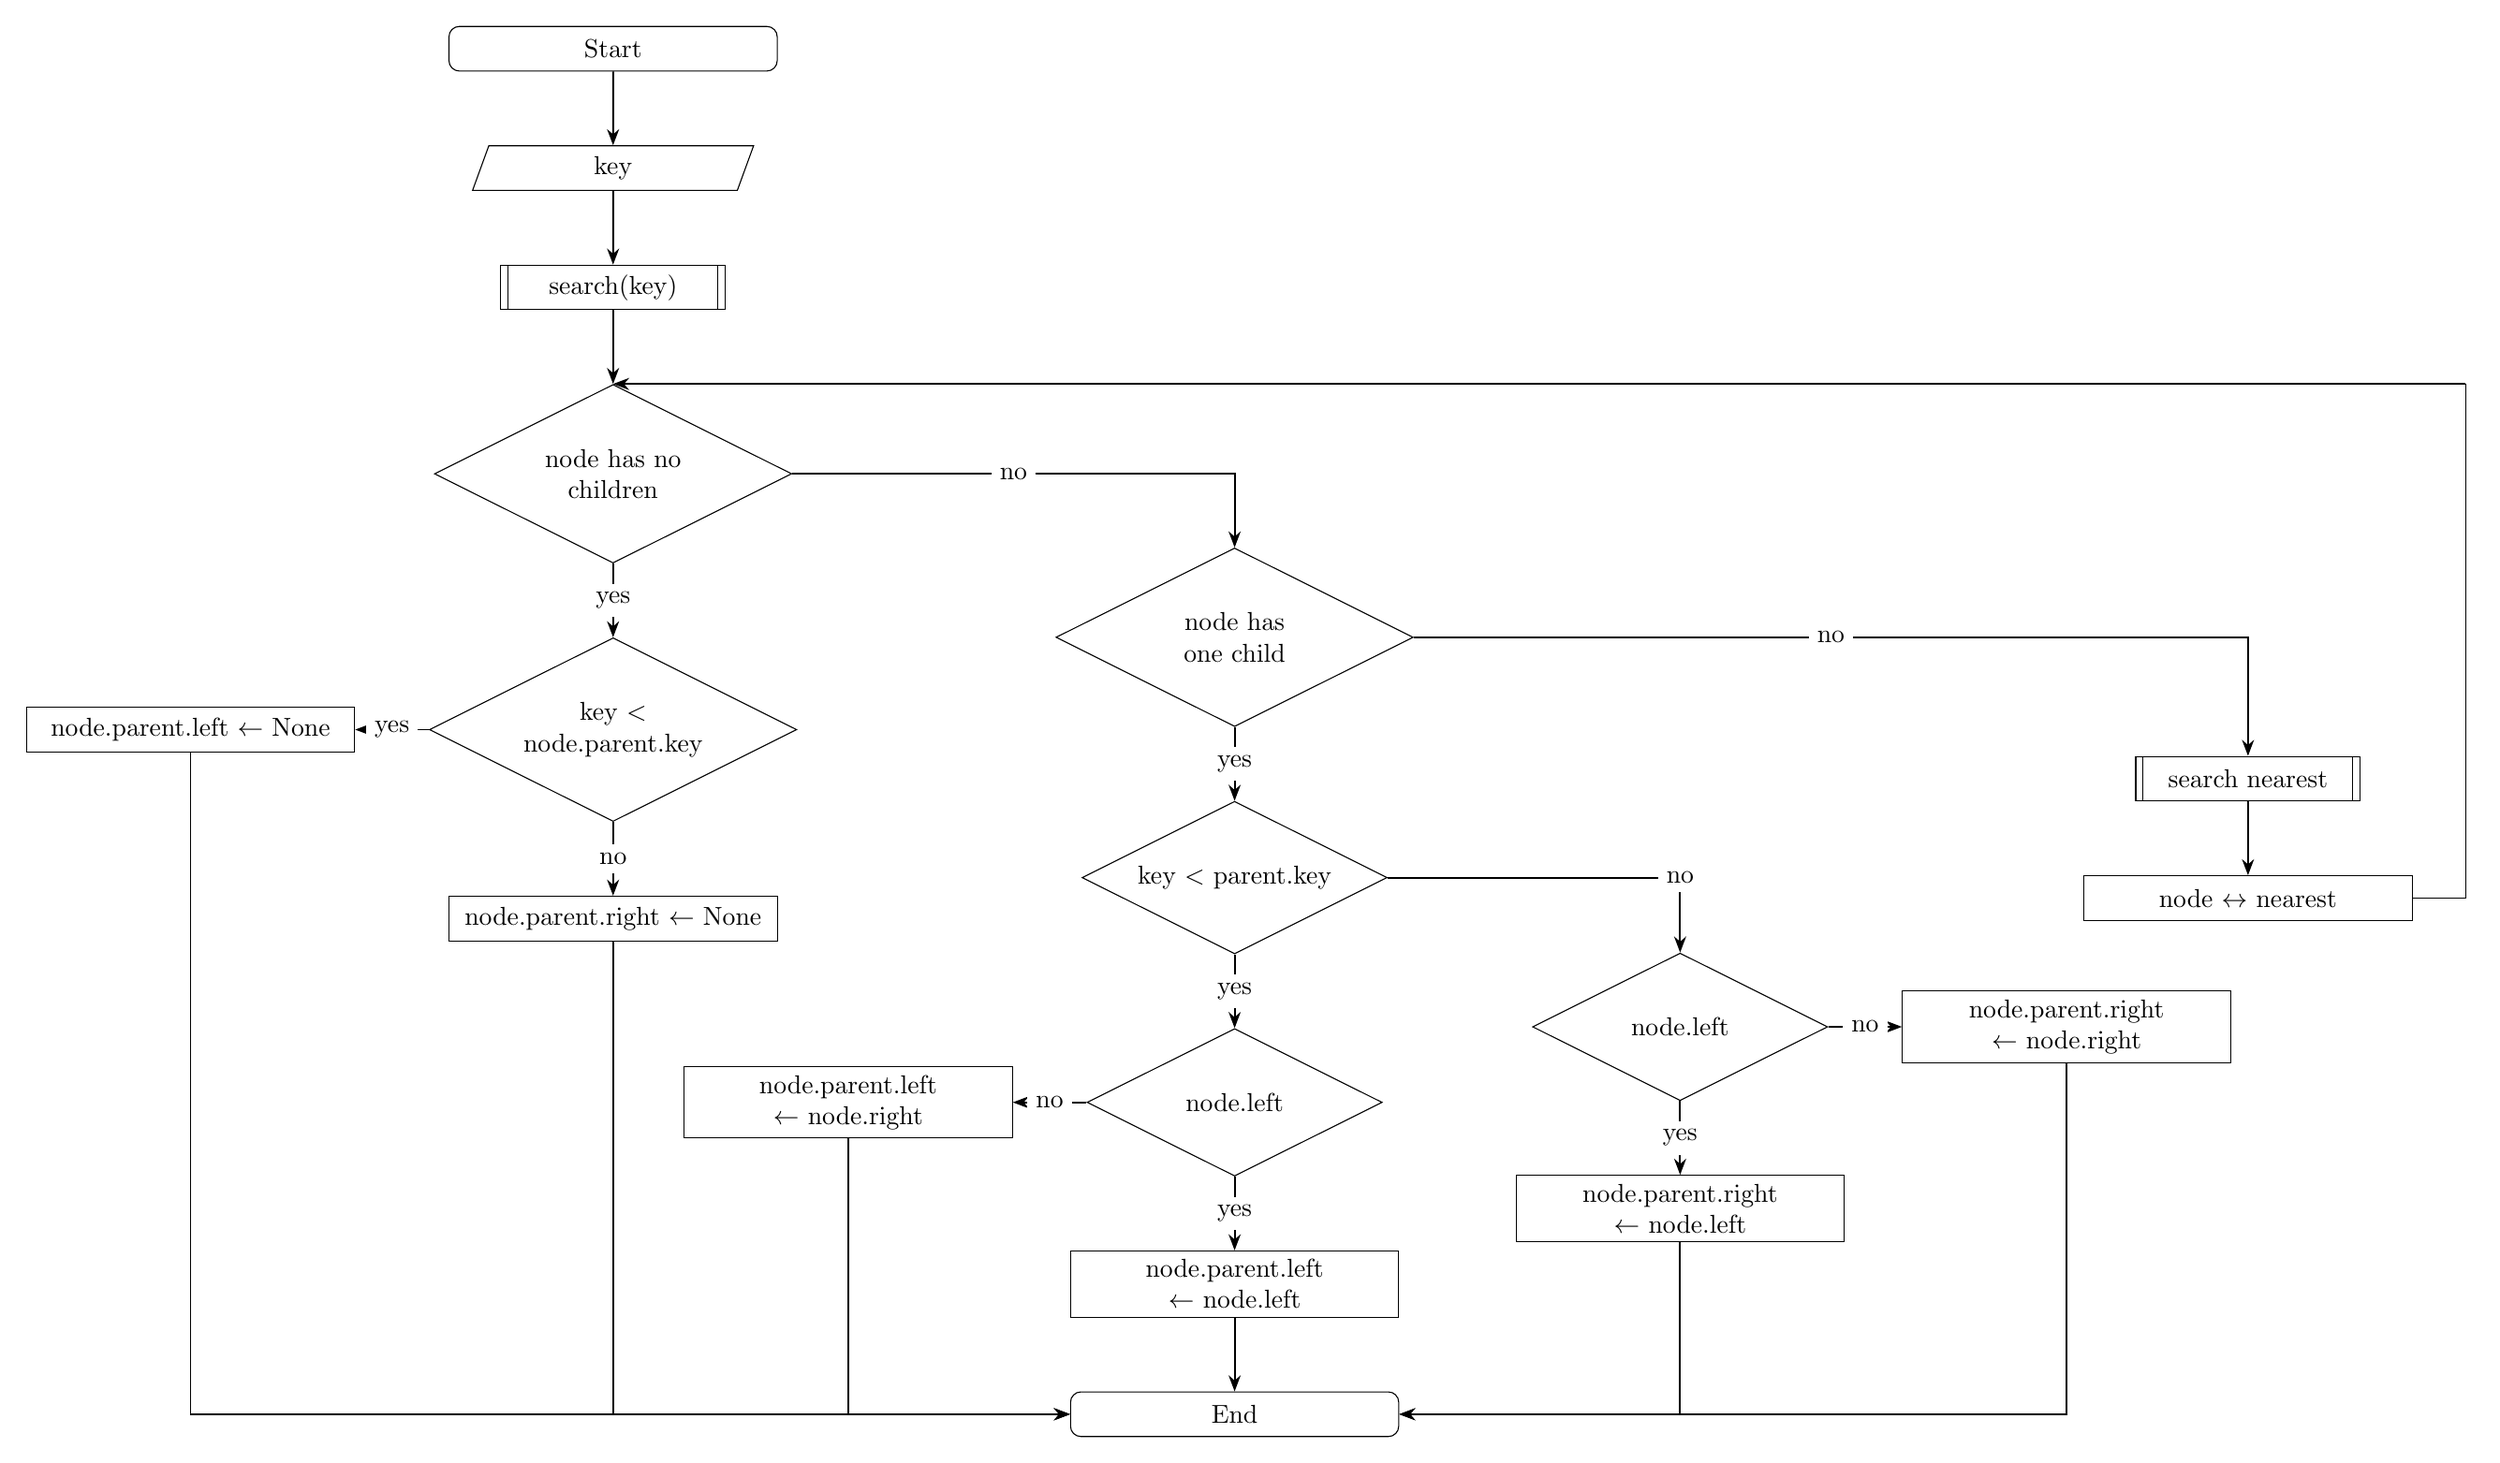
\begin{tikzpicture}
	\node[term] (start) {Start};
        \node[io, below = of start] (input) {key};
        \node[subproc, below = of input] (search) {search(key)};
        \node[test, below = of search] (case1) {node has no children};
        \node[test, below right = of case1, xshift=5cm] (case2) {node has one
        child};
        \node[subproc, below right = of case2, xshift=10cm] (search2) {
              search nearest
              };
        \node[test, below = of case1] (case11) {key $<$
        node.parent.key};

        \node[proc, left = of case11] (d101) {
              node.parent.left $\leftarrow$ None};
        \node[proc, below = of case11] (d102) {
              node.parent.right $\leftarrow$ None};

        \node[test, below = of case2] (case21) {key $<$ parent.key};
        \node[test, below = of case21] (case22) {node.left};
        \node[proc, below = of case22] (d211) {
              node.parent.left $\leftarrow$ node.left
        };
        \node[proc, left = of case22] (d212) {
              node.parent.left $\leftarrow$ node.right
        };

        \node[test, below right = of case21, xshift=3cm] (case23) {node.left};
        \node[proc, below = of case23] (d231) {
              node.parent.right $\leftarrow$ node.left
        };
        \node[proc, right = of case23] (d232) {
              node.parent.right $\leftarrow$ node.right
        };

        \node[proc, below = of search2] (change) {node $\leftrightarrow$
        nearest};

        \node[right = of case1.north, xshift=24cm] (h1) {};

        \node[term, below = of d211] (end) {End};

        \draw[myarrow] (start) -- (input);
        \draw[myarrow] (input) -- (search);
        \draw[myarrow] (search) -- (case1);
        \draw[myarrow] (case1) -- node[fill=white] {yes} (case11);

        \draw[myarrow] (case11) -- node[fill=white] {yes} (d101);
        \draw[myarrow] (case11) -- node[fill=white] {no} (d102);

        \draw[myarrow] (case1) -| node[near start, fill=white] {no} (case2);
        \draw[myarrow] (case2) -- node[fill=white] {yes} (case21);
        \draw[myarrow] (case21) -- node[fill=white] {yes} (case22);
        \draw[myarrow] (case22) -- node[fill=white] {yes} (d211);
        \draw[myarrow] (case22) -- node[fill=white] {no} (d212);
        \draw[myarrow] (case21) -| node[fill=white] {no} (case23);
        \draw[myarrow] (case23) -- node[fill=white] {yes} (d231);
        \draw[myarrow] (case23) -- node[fill=white] {no} (d232);

        \draw[myarrow] (case2) -| node[near start, fill=white] 
             {no} (search2);

        \draw[myarrow] (search2) -- (change);

        \draw (change) -| (h1.center);
        \draw[myarrow] (h1.center) -- (case1.north);

        \draw[myarrow] (d101) |- (end);
        \draw[myarrow] (d102) |- (end);
        \draw[myarrow] (d212) |- (end);
        \draw[myarrow] (d231) |- (end);
        \draw[myarrow] (d232) |- (end);
        \draw[myarrow] (d211) -- (end);


\end{tikzpicture}
\end{document}
